\section{Week 3}
\subsection{Objective}
This week, we will study and implement the variational inference framework with the objective of
estimating the posterior in a way that is indifferent to the type of regression performed.
We are going to pose the problem as an optimization problem and then derive an objective function that we can optimize over.
We will then try to implement it and perform some adjustments for efficiency and numerical stability.
% The objective of this week is to learn about and implement variational inference for Bayesian linear regression. 
% Then we will study convergence rates and accuracy by playing around with different parameters.
\subsection{Theory}
\subsubsection{Variational Inference and Variational Families}
In week 1, we were able to calculate the exact posterior using the right assumption and conjugacy between the prior and likelihood.
This turns out to be a rarity - in most cases, a closed form solution for the posterior is not readily available.
A common approach to this problem is to approximate the posterior distribution, using a \textit{variational distribution} $q$ picked from a family of distributions 
that we might imagine could approximate the posterior.
By picking a suitable objective function, we can use optimization techniques to approximate the posterior.
This is called \textit{variational inference}.
\\
The point of variational inference is to approximate the posterior distribution $p(\theta | \B{y}, \B{d})$ using optimization techniques.
The space of which to optimize in is the parameter space for some distribution $q(\theta)$, which we aim to make as close to the posterior as possible by KL-divergence.
For reference, we will recite the definition of our linear model:
$$\theta \sim \mathcal{N}(\B{\mu}, \B{\Sigma})$$
$$\epsilon \sim \mathcal{N}(0, \sigma^2_\B{y})$$
$$\B{y} | \B{d}, \theta \sim \theta^T \B{d} + \epsilon$$
The optimization problem we wish to solve is defined like so:
$$q^*(\theta) = \arg \min_{q(\theta) \in \mathcal{L}} \textsc{KL}(q(\theta) || p(\theta | \B{y}, \B{d}))$$
Computing the KL-divergence is hard though, because it requires computing the evidence $p(\B{y}, \B{d})$\todo{show why}, so instead we try to optimize in regards to the expectation lower bound (ELBO):
$$\textsc{ELBO}(q) = \mathbb{E}_{\theta'}[\log p(\theta', \B{d}, \B{y})] - \mathbb{E}_{\theta'}[\log q(\theta')]$$
Let us pick $q(\theta')$ from the family of multivariate normal distributions. This is reasonable, since we expect the posterior to be normally distributed due to conjugacy between the prior and likelihood.\\
It is possible to rewrite the ELBO into a shape that is easier to optimize:
$$\textsc{ELBO}(q) = \mathbb{E}_{\theta'}[\log p(\theta', \B{d}, \B{y})] - \mathbb{E}_{\theta'}[\log q(\theta')]$$
$$ = \mathbb{E}_{\theta'}[\log p(\B{y} | \theta', \B{d}) p(\theta' | \B{d})p(\B{d})] - \mathbb{E}_{\theta'}[\log q(\theta')]$$
$$ = \mathbb{E}_{\theta'}[\log p(\B{y} | \theta', \B{d}) + \log p(\theta' | \B{d}) + \log p(\B{d})] - \mathbb{E}_{\theta'}[\log q(\theta')]$$
$$ = \mathbb{E}_{\theta'}[\log p(\B{y} | \theta', \B{d})] + \mathbb{E}_{\theta'}[\log p(\theta' | \B{d})] + \mathbb{E}_{\theta'}[\log p(\B{d})] - \mathbb{E}_{\theta'}[\log q(\theta')]$$
$$ = \mathbb{E}_{\theta'}[\log p(\B{y} | \theta', \B{d})] + \mathbb{E}_{\theta'}[\log p(\theta')] - \mathbb{E}_{\theta'}[\log q(\theta')] + \const$$
$$ = \mathbb{E}_{\theta'}[\log p(\B{y} | \theta', \B{d})] - (-\mathbb{E}_{\theta'}[\log p(\theta')] + \mathbb{E}_{\theta'}[\log q(\theta')]) + \const$$
$$ = \mathbb{E}_{\theta'}[\log p(\B{y} | \theta', \B{d})] - \mathbb{E}_{\theta'}[\log \frac{q(\theta')}{p(\theta')}] + \const$$
$$ = \mathbb{E}_{\theta'}[\log p(\B{y} | \theta', \B{d})] - \textrm{KL}(q || p) + \const$$
Since $q$ and $p$ are multivariate normal by assumption, we can use the closed-form solution for $\textrm{KL}(q || p)$. 
Thus, we only need to worry about the first part of the expression, which is an integral over the likelihood.\\
Now, we need to use the assumption about the multivariate normal distribution, that the covariance matrix must satisfy $\Sigma = AA^T$ for some matrix $A$ \todo{add this assumption to week 1}.
This means that
$$\theta \sim \mathcal{N}(\mu_\theta, A_\theta A_\theta^T)$$
$$\theta = \mu_\theta + A_\theta z$$\todo{why? (see eq 25 from lecture notes)}
where
$$z \sim \mathcal{N}(0, 1)$$
Thus we can rewrite our ELBO function as
$$\textsc{ELBO}(q) = \mathbb{E}_{z}[\log p(\B{y} | \mu_\theta + A_\theta z, \B{d})] - \textrm{KL}(q || p) + \const$$
thus the log-likelihood is independent of $\theta'$.\\
Now consider the first expectation:
$$\mathbb{E}_{z}[\log p(\B{y} | \mu_\theta + A_\theta z, \B{d})]$$
$$=\int_{z}p(z) \log p(\B{y} | \mu_\theta + A_\theta z, \B{d})\ dz$$
$$\approx \frac{1}{N}\sum_{i=1}^N p(z^{(i)})\log p(\B{y} | \mu_\theta + A_\theta z^{(i)}, \B{d})$$
where $N \in \mathbb{Z}$ and $z_i \sim \mathcal{N}(0, 1)$.
% \subsubsection{Questions for Oswin, May 15}
% \begin{itemize}
%   \item In the current form, I still need to calculate the log-likelihood $\log p(\B{y} | \mu_\theta + A_\theta z^{(i)}, \B{d})$. Since this depends on $\mu_\theta$ and $A_\theta$, when we optimize for $\mu_\theta$ and $A_\theta$\\
%     we're going to calculate (by autograd)
%     $$\nabla_{\mu_\theta, A_\theta} \frac{1}{N}\sum_{i=1}^N p(z^{(i)})\log p(\B{y} | \mu_\theta + A_\theta z^{(i)}, \B{d})$$
%     $$= \frac{1}{N}\sum_{i=1}^N p(z^{(i)})\nabla_{\mu_\theta, A_\theta}\log p(\B{y} | \mu_\theta + A_\theta z^{(i)}, \B{d})$$
%     From our assumption that the likelihood is normally distributed, we thus have that
%     $$= \frac{1}{N}\sum_{i=1}^N p(\B{z}^{(i)})\nabla_{\mu_\theta, A_\theta}\log \mathcal{N}(\B{y} ; \mu_\theta + A_\theta \B{z}^{(i)}, \sigma^2_\B{y}I)$$
%     (by lecture notes, page 31). Thus, we need to compute the gradient of the normal distribution, which Autograd do not support, even using \texttt{autograd.scipy.optimize}, due to passing Arrayboxes into the mean-parameter.
% \end{itemize}
% Now we can estimate the expectation by averaging over different values of the log-likelihood from samples of $z$.

% \subsubsection{Main points from meeting}
% \begin{itemize}
%   \item Let us move away form Mean-field family - we can just pick $q(\theta)$ to be a multivariate normal distribution.
%     We are going to optimize to find the location and covariance.
%   \item It is possible to refactor the ELBO to an expression of the shape
%     $$ELBO(q) = \mathbb{E}_\theta' [\log p(\B{y}| \B{\theta}', \B{d})]- \textsc{KL}(q||p)$$
%     Since $q$ and $p$ are both multivariate normal distributions, we know the KLD is a closed-form solution.
%   \item Use a reparameterization trick (?) of using the assumption $\Sigma = AA^T$ such that $\theta = \mu_\theta + Az$ where $z\sim \mathcal{N}(0, I)$ to change $\mathbb{E}_\theta'[\log p(\B{y}| \theta', \B{d})]$ to $\mathbb{E}_z[\log p(\B{y}| \mu_\theta + Az, \B{d})]$.\\
%     Sample some amount of $z$'s, calculate the inner part of the expectation and average it (i.e. sample from the integral).
%   \item We need to use Stochastic optimization and I probably need to implement that part myself.
% \end{itemize}
\subsection{Design}
The implementation is heavily utilizes the \texttt{autograd} library, which automatically calculates the gradient of the ELBO.
To do this, it was nescessary to manually implement the PDF for the likelihood, since the one provided by Autograd doesn't support optimizing over the mean of the distribution.\\
Several measures were taken to ensure numerical stability in this implementation including using the log-sum-exp trick as well as using the logarithm of the determinant instead of the actual determinant.
It is also nescessary to make sure that enough samples are drawn of $\B{z}$ to ensure our expectation over the log-likelihood is accurate enough. 100 samples were used in this implementation.
Another issue that arises is that sometime the log-likelihood becomes a very small negative number (often denoted as $-\infty$ by Numpy). This happens when a sample $z$ is picked such that the log-likelihood $p(\B{y}| \mu_\theta + A_\theta z^(i), \B{d})$ becomes very close to zero.
This was solved by simply rejecting any sample that results in such a log-likelihood.

Another problem that arises is overflows when the amount of datapoints become larger.
To handle this, it first of all makes sense to work directly with the log of the likelihood instead of first calculating the likelihood and then taking the log of it.
$$-\frac{1}{2}(n \log(2\pi) + \log(\det(\Sigma)) + (x-\mu)^T \Sigma^{-1}(x-\mu))$$ \todo{Why is logpdf true? prove in theory}
This also means that we don't need to apply the log-sum-exp trick, since we are working directly with logarithms.
A disadvantage with this method is first of all that we can't guarantee that the covariance has an inverse, and secondly that computing the inverse of large matrices is very inefficient.
To solve the first issue, we can try regularize the covariance matrix by adding a small constant to the diagonal.
The second could potentially be solved by using some sort of approximation like Cholesky decomposition, but this was not regarded for now.
The stop condition for the optimization is decided by the default gradient tolerance of the scipy-implementation, 
but in practice the optimization is stopped when the precision of the gradient is lost due to the stocastic nature of the objective function.
This typically happens when trying to take small steps around the minimum, but as can be seen in Figure ... the precision is increased when the amount of datapoints is increased.
\subsection{Results}\todo{Make subplots}
\begin{figure}[H]
  \centering
  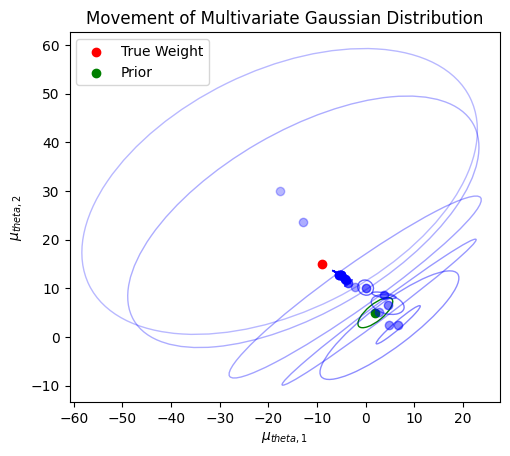
\includegraphics[width=\textwidth]{week3/ellipses.png}
  \caption{Optimization over the ELBO for 50 datapoints}
\end{figure}
\begin{figure}[H]
  \centering
  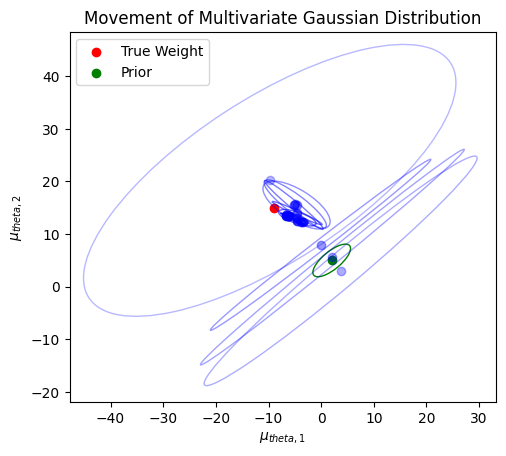
\includegraphics[width=\textwidth]{week3/ellipses-100.png}
  \caption{Optimization over the ELBO for 100 datapoints}
\end{figure}
\begin{figure}[H]
  \centering
  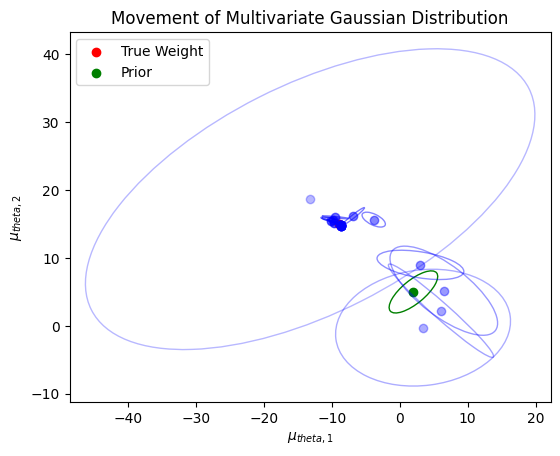
\includegraphics[width=\textwidth]{week3/ellipses-300.png}
  \caption{Optimization over the ELBO for 300 datapoints}
\end{figure}
\begin{figure}[H]
  \centering
  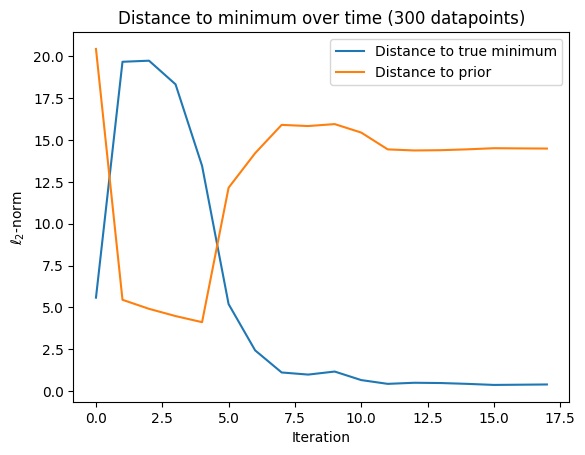
\includegraphics[width=\textwidth]{week3/Distance to minimum-300.png}
  \caption{Optimization over the ELBO for 300 datapoints}
\end{figure}
As one can see, the optimization converges quite close to the true weights when the amount of datapoints increases as expected.
First, the algorithm quickly moves towards the prior, and then slowly moves towards the true minimum. 
If the prior is close to the true minimum, one could expect that the algorithm would converge faster.
It is also seen that the covariance of the parameters quickly become very small. \todo{Interpret this - what does that mean?}
\subsection{Evaluation}
The algorithm presented here seems to work - although it is not as efficient as the analytical solution, it represents a framework that could be more useful for other problems.
From this we've also learned a bit about how we can expect the movement of the distribution - first towards the prior, then towards the minimum.
It has also shown the importance of numerical stability as well as how we can use the reparameterization trick for efficient computation.
